\subsubsection{F.2.2 Calculate Train Position}\label{sss:calctrainpos}

\paragraph{Short Description of Functionality}
The main purpose of the function is to calculate the locations of linked and unlinked balise groups (BGs) and the current train position while the train is running along the track. 

In detail, the calculateTrainPosition function provides a couple of essential subfunctions for the onboard unit. These are mainly
\begin{itemize}
\item creating and maintaining an obu internal coordinate system for all types of location based data
\item storing all linked and unlinked balise groups resulting from over passing or from announcements (linking information) from the track
\item calculating and maintaining the locations of all stored balise groups during the train trip, based on odometry and linking information
\item permanently calculating the current train position based on odometry and passed balise group information
\item providing the last recently passed linked balise group as the LRBG
\item providing additional position attribute information
\item deleting stored balise groups, when appropriate
\item detecting linking consistency errors
\item determining, if linking is used on board
\end{itemize}

\newpage

The calculation algorithms for locations and positions are implemented as specified in 
\url{https://github.com/openETCS/SRS-Analysis/blob/master/System%20Analysis/WorkingRepository/Group4/SUBSET_26_3-6/DetermineTrainLocationProcedures.pdf} .

\begin{figure}[!htb]
\centering
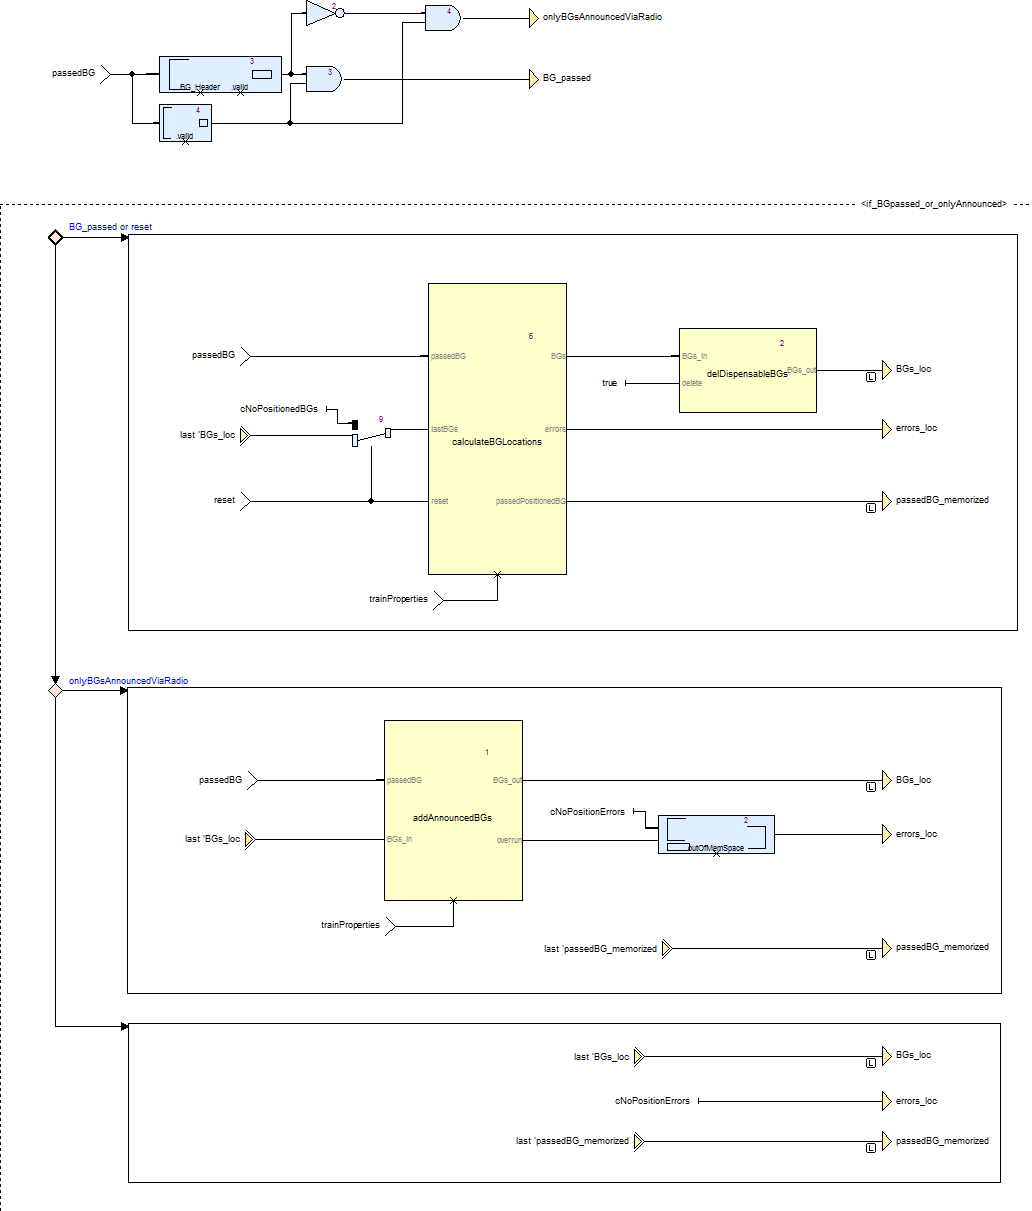
\includegraphics[scale=0.5]{../images/calculateTrainPosition_calcBGs.png}
\caption{Calculating the balise group locations}
\end{figure}
\clearpage

\begin{figure}[!htb]
\centering
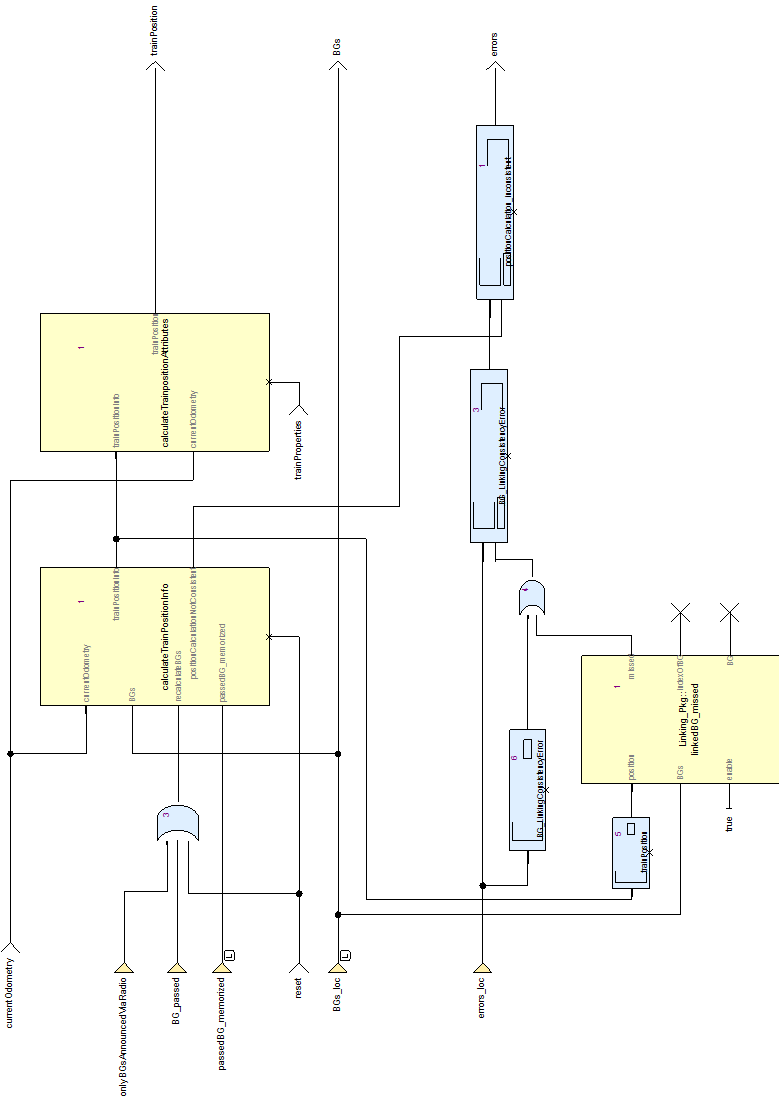
\includegraphics[scale=0.5]{../images/calculateTrainPosition_decorations.png}
\caption{Calculating the current train position and attributes}
\end{figure}

\clearpage

\paragraph{Functional Structure in Stages}
calculateTrainPositions receives its input information via its passedBG entry as an event. The first decicion to be made is, if an input event is available and if it origins from a balise group just over passed or from the RBC via radio. 

If the passedBG input events is caused by over passing a balise group, the balise group gets an OBU coordinate system location assigned ("calculateBGLocations") and is stored internally. If the just passed balise group announces more balise groups ahead via linking, they are stored with their locations calculated. 

If the passedBG input event origins from RBC data received ("addAnnouncedBGs"), it only announces balise groups ahead. These announced balise groups get their locations calculated with reference to the LRBG and are stored as well.

"calculateBGLocations" and "addAnnouncedBGs" produce a list of known balise groups ("BGs"). 

The following stages "calculateTrainPositionInfo" and "calculateTrainpositionAttributes" all the time calculate the current train position by using the list of known balise groups (including the LRBG) and the current odometry information and determine additional position attributes.

In parallel "linkedBG\_missed" is part of linking consistency supervision. It detects, when an announced balise group is not found within its expectation window. 

In more detail, "calculateTrainPosition" is divided into a data flow of different stages, which are being performed sequentially: 
\begin{enumerate}
\item \textbf{\textit{calculateBGLocations}}: Calculate the balise group locations\\
The  stage is triggered each time the train passes a balise group (input \textit{passedBG}). It takes the balise group header with the BG identification, the linking information (Subset 26, packet 5) and the current odometry values as inputs and calculates the location of the passed balise group. If the passed BG has been announced via linking information previously, it takes into account the linking as well as the odometry information. If the passed BG does not meet the expectation window announced by linking, an error flag is set. If the passed BG is an unlinked BG, its location is determined by odometry only, but related to the next previously passed linked BG (LRBG), if there is one.\\
Then, if the passed BG is a linked BG comprising linking information for BGs ahead, the linking information is evaluated by creating the announced BGs and computing their locations from the linking distances.\\
The passed and the announced BGs are stored in a list \textit{BGs} in the order they are passed and by their announced nominal location on the track.\\
Afterwards the locations of all BGs are further improved by re-adjusting their locations with reference to the just passed BG. This optimizes the BG location inaccuries around the current train position (= location of the passed BG). 

\item \textbf{\textit{delDispensableBGs}}: Delete dispensable balise groups\\
The function removes balise groups supposed not to be needed any longer from the list of \textit{BGs}.\\
If the number of stored passed linked BGs exceeds the maximum number as specified in \cite[Chapter~3.6.2.2.2 c]{subset-026}, all BGs astern are deleted.
If only (passed) unlinked BGs are in the list and exceed the number of \textit{cNoOfAtLeast\_x\_unlinkedBGs}, all passed BGs astern to those are removed from the list. 

\item \textbf{\textit{addAnnouncedBGs}}: This function is executed once each time balise groups ahead are announced by the RBC. The locations of the announced \textit{BGs} are calculated with reference to the LRBG reported by the RBC. 

\item \textbf{\textit{calculateTrainPositionInfo}}: Calculate train position information.\\
This stage takes the list of stored BGs and the current odometry values as inputs and steadily provides the current train position. Additionally, it watches the list of announced \textit{BGs} and provides the "Linking information is used" information as specified in chapt. 3.4.4.2.1.1 of the SRS. 

\item \textbf{\textit{calculateTrainpositionAttributes}}: Calculate train position attribute information.\\
This stage provides several additional position related attributes that might conveniently be used by subsequent consumers in the architecture. It in addition provides the current LRBG and the previous LRBG from the list \textit{BGs}. 

\item \textbf{\textit{linkedBG\_missed}}: This function observes the list of \textit{BGs} and the current train position. If an announced balise group is not found within its expectation window, an error flag will be raised. 

\end{enumerate}


\paragraph{Reference to the SRS (or other requirements)}
The component calculateTrainPosition determines the location of linked and unlinked balise groups and the current train position during the train trip as specified mainly in \cite[Chapter~3.6]{subset-026}.

\paragraph{Design Constraints and Choices}
The following constraints and prerequisites apply:
\begin{enumerate}
\item The input data received from the balises groups or via radio must have been checked and filtered for validity, consistency and the appropriate train orientation before delivering them to calculateTrainPosition. 
\item The storage capacity for balise groups is finite. calculateTrainPosition will raise an error flag when a balise group cannot be stored due to capacity limitations.
\item calculateTrainPosition will raise an error flag if a just passed balise group is not found where announced by linking information or if an announced balise group is missed when the end of its expectation window is reached. It does not yet implement all conditions of linking consistency.
\item calculateTrainPosition is not yet prepared for train movement direction changes. 
\item calculateTrainPosition does not yet consider repositioning information.
\end{enumerate}



\subsubsection{Provide Position Report}\label{sss:provposrep}

\begin{figure}[ht]
\centering
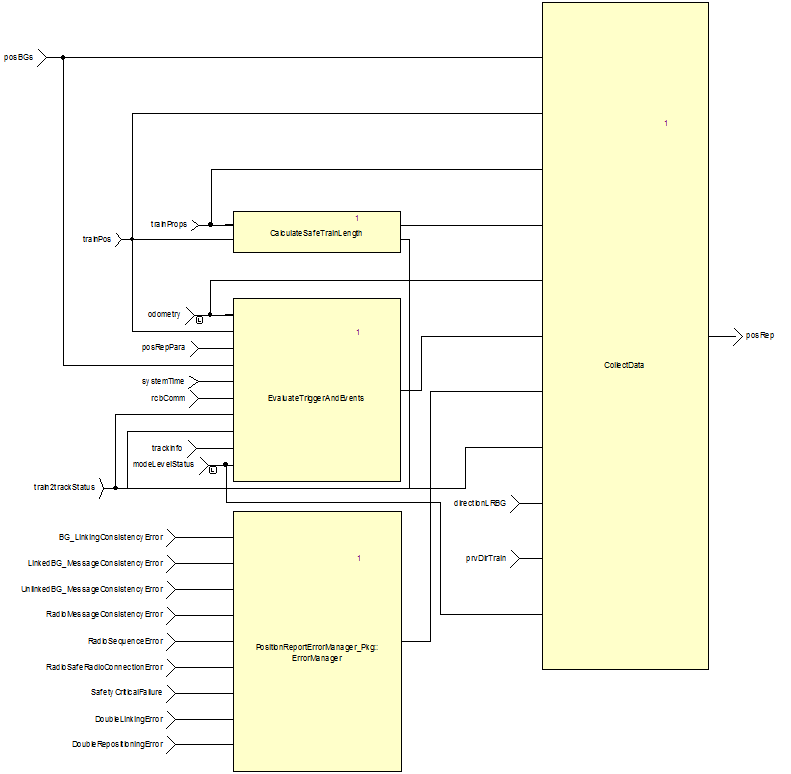
\includegraphics[width=\textwidth]{../images/ProvidePositionReport.PNG}
\caption{Structure of component ProvidePositionReport}\label{fig:provideposrep}
\end{figure}

\paragraph{Short Description of Functionality}
This function takes the current train position and generates a position report which is sent to the RBC. The point in time when such a report is sent is determined by events, on the one hand, and position report parameters---which are basically triggers---provided by the RBC or a balise group passed, on the other hand. The functionality is modeled using four operators, as shown in Figure~\ref{fig:provideposrep}, which are explained below.
\begin{description}
	\item[CalculateSafeTrainLength] Calculates the the safeTrainLength and the MinSafeRearEnd according to \cite[Chapter~3.6.5.2.4/5]{subset-026}. \\
\verb+safeTrainLength =  absolute(EstimatedFrontEndPosition - MinSafeRearEnd)+, where
\verb+MinSafeRearEnd = minSafeFrontEndPosition - L_TRAIN+.
	\item[EvaluateTriggerAndEvents] Returns a Boolean modelling whether the sending of the next position report is triggered or not. This value is the conjunction of the evaluation of all triggers (PositionReportParameters, i.e., Packet 58) and events (see \cite[Chapter~3.6.5.1.4]{subset-026}).
	\item[ErrorManager] Takes a boolean flag for each possible error that has been occurred and outputs the respective error using type \verb+M_ERROR+
	\item[CollectData] This operation aggregates data of Packet 0, \dots, Packet 5 and the header to a position report.
\end{description}

\paragraph{Reference to the SRS (or other requirements}
Most of the functionality is described in \cite[Chapter~3.6.5]{subset-026}.

\paragraph{Design Constraints and Choices}
\begin{enumerate}
	\item The message length (i.e., attribute \verb+L_MESSAGE+) is by default set to 0; the actual value will be set by the Bitwalker/API.
	\item The attribute \verb+Q_SCALE+ is assumed to be constant; that is, all operations using this attribute do not convert between different values of that attribute.
	\item \textit{PositionReportHeader}: The time stamp (i.e., attribute \verb+T_TRAIN+) is not set; this should be done once the message is being sent by the API.
	\item \textit{Packet 4}: When aggregating data for this packet, an error message might be overwritten by a succeeding error message. Because the specification allows only to sent one error in one position report, errors are not being stored in a queue, for instance.
	\item \textit{Packet 44}: This packet is currently not contained in a position report as it is not part of the kernel functions.
	\item The usage of attributes \verb+D_CYCLOC+ and \verb+T_CYCLOC+ as part of the triggers specified by the position report parameters (i.e., Packet 58 sent by the RBC) may lead to unexpected results if a big clock cycle together with small values for the attributes is used. The cause is that at every clock cycle the current model increments the reference value for the distance and time by at most \verb+D_CYCLOC+ and \verb+T_CYCLOC+, respectively and not a factor of it.
	\item The \textit{ErrorHandler} is currently restricted to deal with a single error. As a consequence, as for each error reported a report has to be sent to the RBC, the number of reports is limited to one.
\end{enumerate}

\paragraph{Open Issues}
\begin{enumerate}
	\item The specification requires to store the last eight balise groups for which a position report has been sent (see \cite[Chapter~3.6.2.2.2.c]{subset-026}).
	\item For all reports that contain Packet 1 (i.e., report based on two balise groups), the RBC sends a coordinate system. It is unclear where this has to be stored (i.e., somehow the balise groups have to be stored in a database which has then to be updated), see \cite[Chapter~3.4.2.3.3.6]{subset-026}. Moreover, such a coordination system can be invalid and then has to be rejected (see \cite[Chapter~3.4.2.3.3.7-8]{subset-026}). On a more abstract level, we need to think about the interface between the RBC and the OBU or a proper abstraction thereof.
\end{enumerate}
